\chapter{Experimental Setup}
\section{Synchrotron Radiation}
The radiation emitted by a relativistic charged particle, usually electrons, accelerated to a circular orbit through an external magnetic field is called synchrotron radiation. This radiation is polarized and emitted tangential to the circular movement of the charged particle in forward direction. In the history of synchrotron radiation sources have evolved from parasitic use at particle accelerators to the extend of building electron storage rings dedicated for the sole purpose of generating this radiation \cite{munro_chapter_1987}. Its most promitent features are the high brilliance, that is the number of photons per second per unit particle beam cross section and per unit solid angle within $0.1\%$ bandwidth at a specific wavelength, and its huge spectral range of emission. Depending on the energy of the relativistic particles forced on a circular orbit, in modern electron storage rings typically in the order of one to several GeV, the emission covers the range from the terahertz into the hard X-ray regime. The \gls{ptb} operates two laboratories at the dedicated sources \gls{bessy} and the \gls{mls} \cite{brandt_metrology_2007}. The two thrid-generation synchrotron radiation sources provide maximum electron energies of $1.7$ GeV (\gls{bessy}) and $0.6$ GeV (\gls{mls}), respectively. Theoretical emission spectra for a single dipole magnet (\emph{bending magnet}) are shown in Fig.~\ref{ch_exp:fig_experimental_synchrotron_spectra} in comparison to black body radiation.
\begin{figure}
 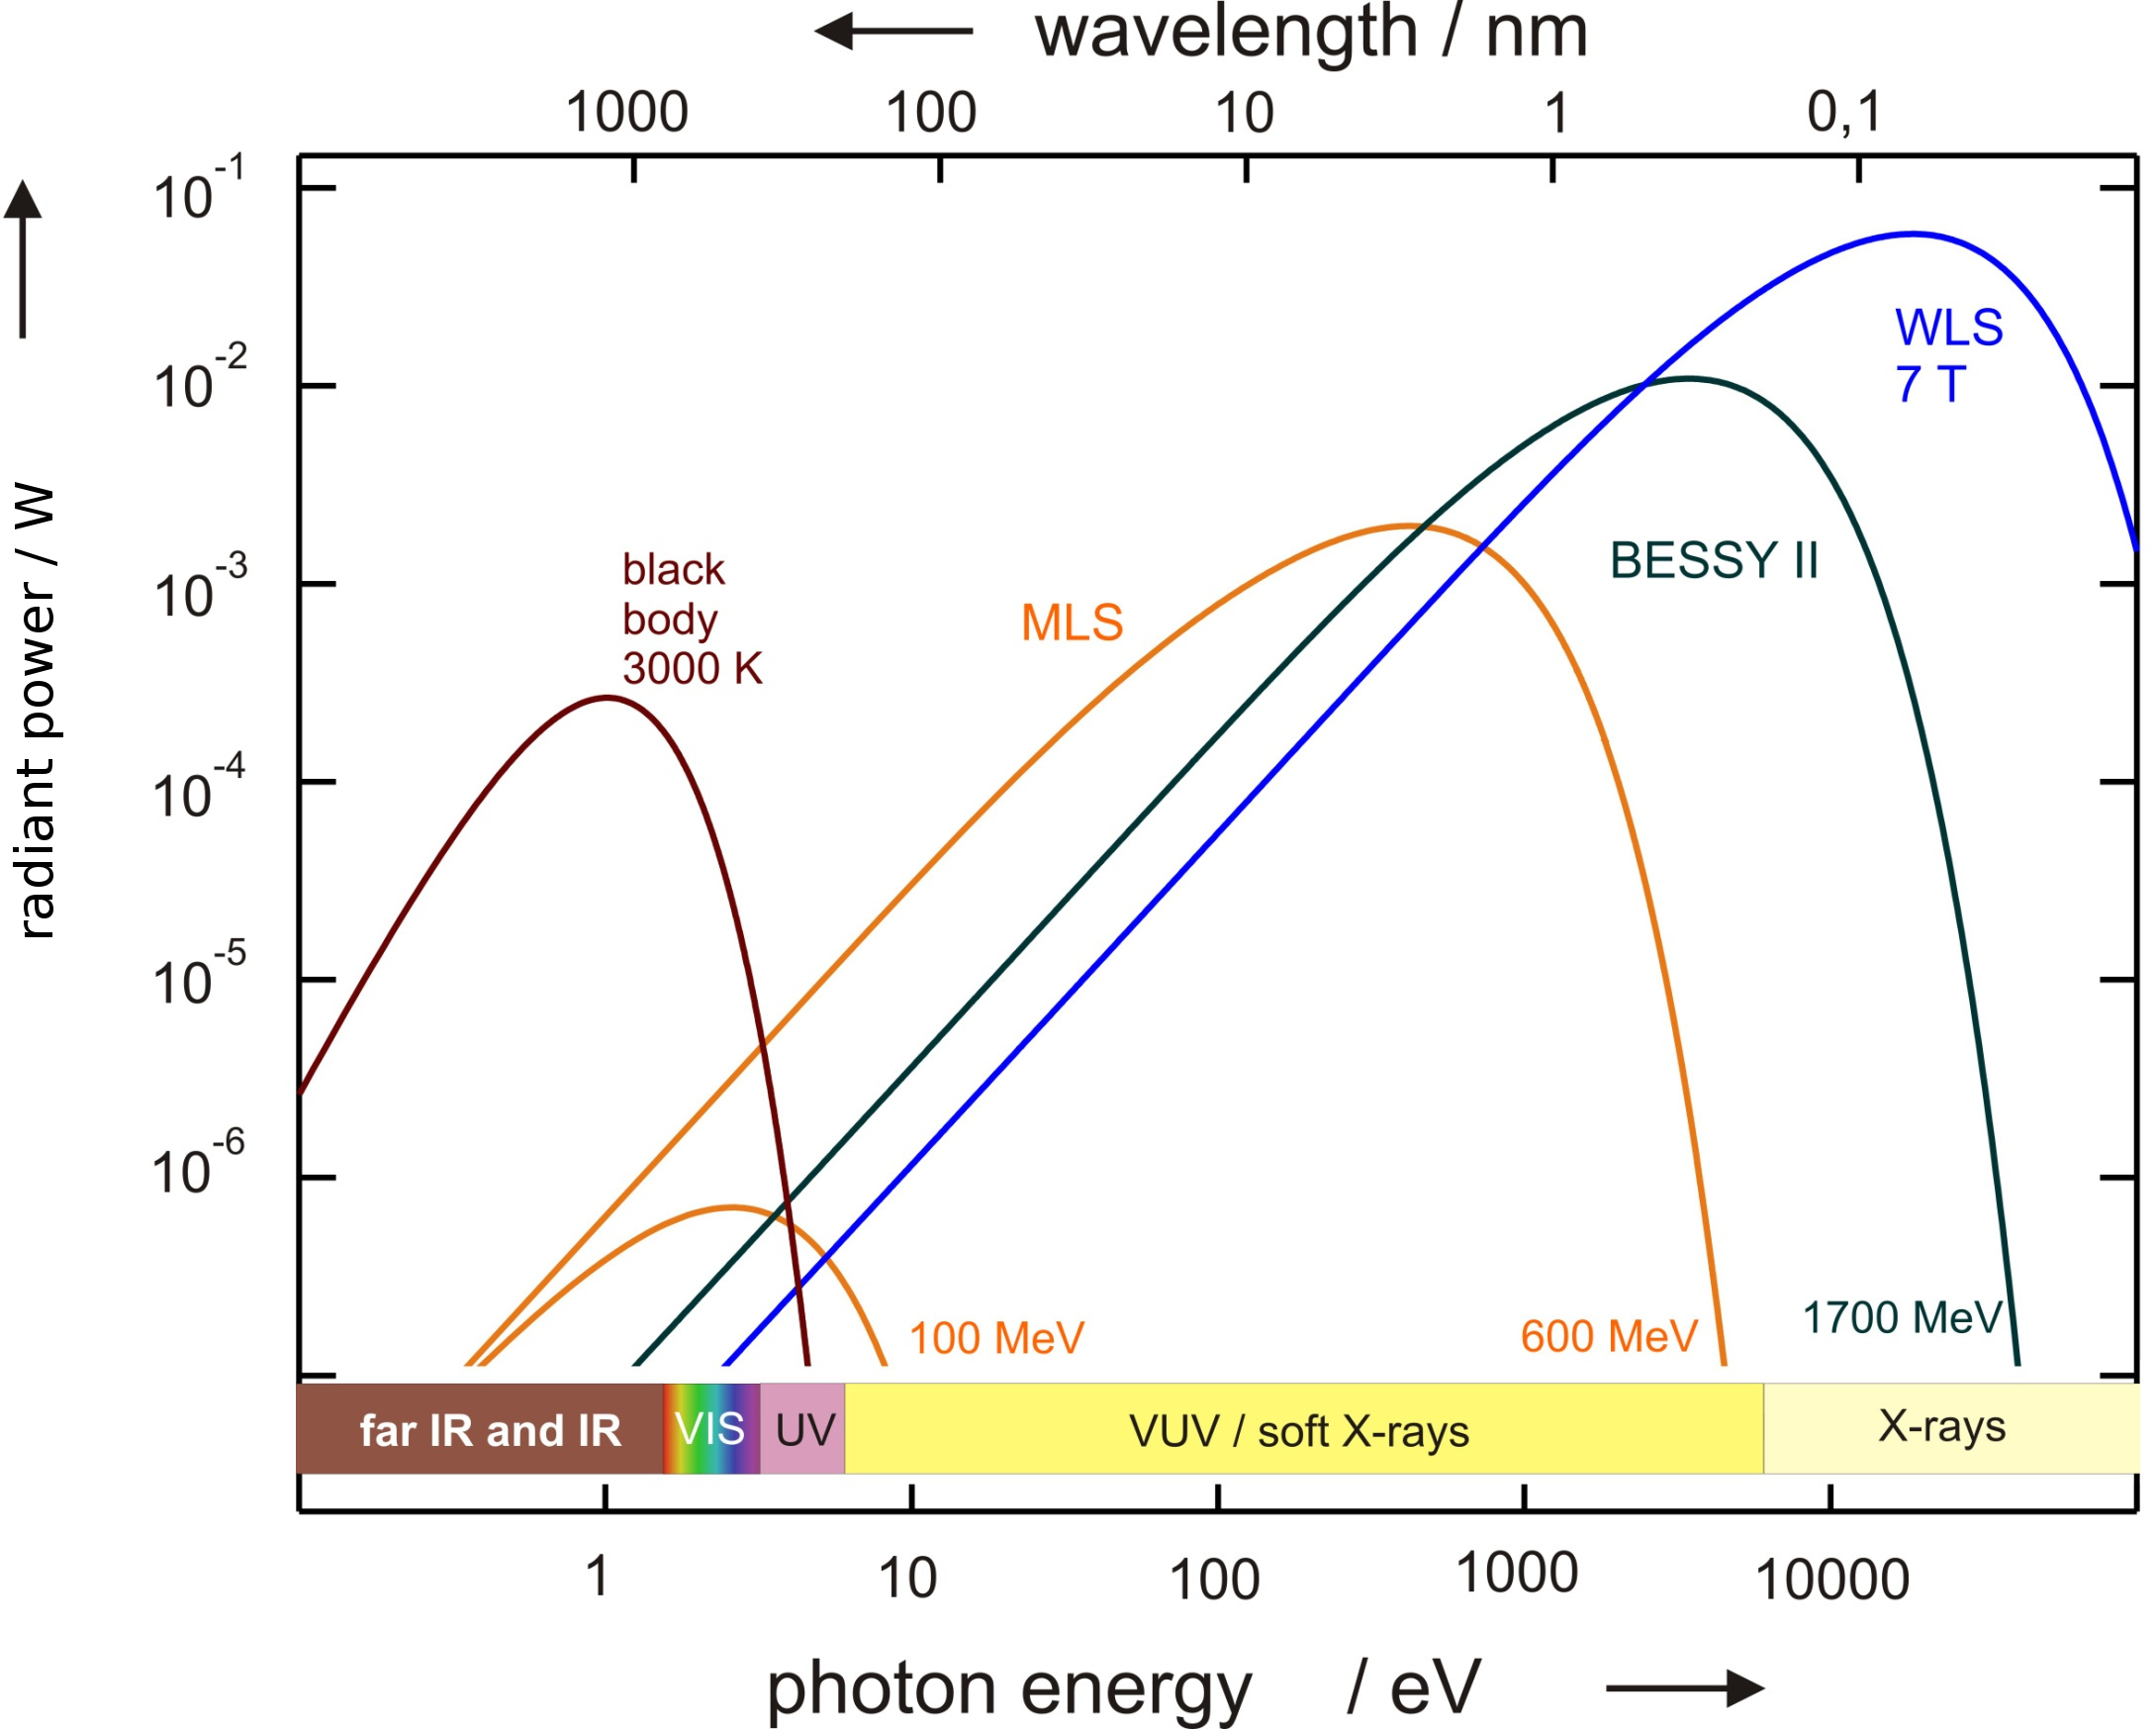
\includegraphics[width=0.7\textwidth]{img/exp-bessy-dipole-spectrum.jpeg}
 \caption[Theoretical synchrotron radiation radiant power spectra]{Theoretical synchrotron radiation radiant power spectra for the \gls{mls} and \gls{bessy} in comparison to black body radiation\footnote{Image taken from Beckhoff et al.~\cite{beckhoff_quarter-century_2009}}. The curves show the radiant power of emission for bending magnets at both electron storage ring facilities for different electron energies. The curve marked WLS shows the radiant power from the $7$ Tesla wavelength shifter insertion device installed at \gls{bessy}.}
 \label{ch_exp:fig_experimental_synchrotron_spectra}
\end{figure}

A very important theoretical aspect of synchrotron radiation, apart from the high brilliance and large spectrum, is the fact that the emission can be calculated exactly from first principles of classical electrodynamics and special relativity. The theory for synchrotron radiation was developed by Schwinger \cite{schwinger_classical_1949} and we shall review its most imporant aspects here. Given all the fundamental and experimental parameters are known, the total emitted radiant power per relativistic particle can be calculated exactly as
\begin{align}
 P = \frac{1}{4 \pi \gls{epsilon_0}} \frac{2}{3} \frac{\gls{e}^2 \gls{c}}{R^2}\Big( \frac{E}{\gls{m_0} \gls{c}^2}\Big)^4 \text{,} \label{ch_exp:schwinger_equation_total_power}
\end{align}
where \gls{e} is the elementary charge, \gls{c} is the speed of light in vacuum, $E$ is the particles energy, \gls{m_0} is the rest mass of the particle and $R$ is the radius of the circular trajectory imposed by the magnetic field. The radiant power is thus inversely proportional to the fourth power of the particles rest mass, which explains the usage of light electrons in comparison with significanlty heavier protons in synchrotron radiation sources. The dependence on the electron energy is visible in another characteristic value for the emitted radiant power, visible as a shift to higher photon energies (smaller wavelengths) in Fig.~\ref{ch_exp:fig_experimental_synchrotron_spectra}, known as the critical energy or critical wavelength \cite{schwinger_classical_1949}, respectively,
\begin{align}
 E_C = \frac{3 \gls{h} \gls{c}}{4 \pi R} \Big( \frac{E}{\gls{m_0} \gls{c}^2}\Big)^3 \text{.} \label{ch_exp:characteristic_energy}
\end{align}
It marks the point in the spectrum, where the integrated radiant power for all values above and below the critical energy are equal \cite{balerna_introduction_2015}. This formula quantifies the shift towards higher energies due to the increase of the electron energy comparing the \gls{mls} and \gls{bessy} emission spectra. Apart from the spectral distribution, the emitted radiation is linearly polarized with an electric field vector oscillating parallel to the plane of the circular orbit. This property, however, is only stricly valid for the emission inside this plane. For radiation above or below, a vertical polarization component (parallel to the surface normal of the orbital plane) exsists. The energy $W$ emitted by a single electron on a circular orbit per unit solid angle $\text{d} \Omega$ and per unit angular frequency interval $\text{d} \omega$ is described by
\begin{align}
 \frac{\text{d}^2 W}{\text{d} \Omega \text{d} \omega} &= \frac{\gls{e}^2 R^2}{36 \pi^3 \gls{epsilon_0} \gamma^4} \omega^2 \big(1+ (\gamma \Psi)^2\big)\Big( K_{2/3}^2(\zeta) + \frac{(\gamma \Psi)^2}{1 + (\gamma \Psi)^2} K_{1/3}^2(\zeta)\Big) \text{,} \label{ch_exp:schwinger_equation_spectral}
\end{align}
where $\gamma = \sfrac{E}{\gls{m_0} \gls{c}^2}$ and $\Psi$ is the angle between the orbital plane and the observation direction outside of that plane. The argument of the modified Bessel funktions of second kind $K_{x}(\zeta)$ is defined as
\begin{align}
 \zeta = \frac{R \omega}{3 c \gamma^3} \big(1 + (\gamma \Psi)^2\big)^\frac{3}{2} \text{.}
\end{align}


The ability to calculate the exact emission and polarization properties of synchrotron radiation based on Eq.~\eqref{ch_exp:schwinger_equation_spectral} with a given electron current and aceptance angle have another very valuable side effect for the field of metrology. It enables the use of synchrotron radiation as a primary standard for electromagnetic radiation within the available spectral range, which is in fact exploited by the \gls{ptb} \cite{thornagel_electron_2001} no provide absolute radiometry.

The dedicated sychrotron radiation facilities, such as \gls{bessy} and the \gls{mls} provide additional possibilities of generating synchrotron radiation beyond a simple bending magnet through different instertion devices. Fig.~\ref{ch_exp:fig_bessy2} gives a shematic overview over the storage ring \gls{bessy}. At each of the marked dipole magnets, synchrotron radiation is produced according the theory presented above. The radiation is transmitted through outlet systems towards a large number of beamlines, which monochromatize and focus the radiation for experimental applications.
\begin{figure*}[htb]
    \def\svgwidth{0.7\textwidth}
    \import{svg/}{bessy.pdf_tex}
    \caption[Schematic overview of BESSY II.]{Schematic overview of the electron storage ring facility \gls{bessy}\footnote{Original image by \gls{hzb}, Ela Strickert, source: \url{https://www.helmholtz-berlin.de/mediathek/bildarchiv/}}. The synchrotron accelerates the electrons coming from the \gls{linac}, which are then injected in the electron storage ring with their full desired energy. Electromagnetic lenses focus and stabilize the beam, as well as deflecting it onto the circular orbit while emitting synchrotron radiation at each dipole (bending) magnet. Cavities reaccelerate the electrons in the storage ring to compensate the energy loss due to the radiation emission.}
    \label{ch_exp:fig_bessy2}
\end{figure*}
Undulators of wigglers are inserted in the straight sections of the \gls{bessy} storage ring with a large number of periodically arranged magnets with alternating polarization forcing the electrons on a sinosoidal beam path. The goal of these insertion devices is to shift the critical energy of the storage ring towards higher energies (wigglers) or to dramatically increase the brilliance within a significantly smaller spectral range (undulators). The different effects of the undulators and wigglers on the generated spectrum is determined by the magnetic field strength $B_0$ and the distance between two identical periodic arragnements of the magnets of alternating polarization $\lambda_0$. The deflection parameter quantifies this relation through $K \propto B_0 \lambda_0$. Undulators typically have deflection parameters $K < 1$ while in case of wigglers $K \gg 1$ \cite{munro_chapter_1987}. Technically, the magnetic field strength can be varied by changing the distance (``gap'') between the magnets vertically. By changing the vertical alignment of the magnetic field direction with respect to the beam path, it is even possible to affect the polarization properties of the emitted radiation to obtain circularly polarized radiation.

\begin{enumerate}
 \item Schwinger equation per unit solid angle and unit wavelength interval
 \item Free electron lasers. Invention \cite{madey_stimulated_1971}. Demonstration \cite{deacon_first_1977}. Long undulator SASE \cite{derbenev_possibility_1982, bonifacio_collective_1984}
\end{enumerate}

\section{The SX700 and EUVR Beamlines}
\begin{figure*}[htb]
    \def\svgwidth{\textwidth}
    \import{svg/}{exp-ptb-beamlines.pdf_tex}
    \caption[PTB Beamlines in the BESSY II laboratory.]{Beamlines in the laboratory at \gls{bessy}.}
    \label{ch_exp:fig_beamlines_bessy}
\end{figure*}
SX700 \cite{beckhoff_quarter-century_2009}
\section{The ELLI and BigRef Reflectometers}
BigRef \cite{scholze_high-accuracy_2001}
ELLI \cite{soltwisch_polarization_2015}
\section{Grazing-incidence X-ray Fluorescence at the FCM Beamline}

\section{Sample systems}
\begin{enumerate}
 \item Mo/Si mirrors for $13.5$ nm for EUV lithography and other applications
 \item Cr/Sc for the water window, protein contrast in water, mirrors with bad performance, curved, etc.
\end{enumerate}
